% =====================================================================
\section{Teorema del virial}
\label{sec:virial}
% =====================================================================

El virial relaciona los \emph{promedios temporales} de la energía cinética y
de las fuerzas en cualquier movimiento acotado, sin resolver las ecuaciones
de movimiento.

\begin{definicion}[Virial, promedio temporal]
Se definen
\begin{equation}
  S(t)\defeq\sa\vb{r}_{\alpha}\cdot\vb{p}_{\alpha},
  \qquad
  \prom{A}\defeq\lim_{\tau\to\infty}\frac1\tau\int_{0}^{\tau}A(t)\,\dd t .
\end{equation}
Para un movimiento periódico de periodo $T_{0}$ basta promediar sobre un periodo.
\end{definicion}

\begin{teorema}[Virial de Clausius]
\label{teo:virial}
Si todas las $\vb{r}_{\alpha}$ y $\vb{p}_{\alpha}$ están acotadas, con
$\vb{F}_{\alpha}$ la fuerza total sobre $\alpha$,
\begin{equation}
  \resultado{\prom{T}=-\frac12\Bigl\langle\sa\vb{r}_{\alpha}\cdot\vb{F}_{\alpha}\Bigr\rangle} .
  \label{eq:virial}
\end{equation}
\end{teorema}

\begin{proof}
\begin{enumerate}
  \item \emph{Derivar $S$}:
  $\dot S=\sum\dot{\vb{r}}_{\alpha}\cdot\vb{p}_{\alpha}+\sum\vb{r}_{\alpha}\cdot\dot{\vb{p}}_{\alpha}
  =\sum m_{\alpha}v_{\alpha}^{2}+\sum\vb{r}_{\alpha}\cdot\vb{F}_{\alpha}=2T+\sum\vb{r}_{\alpha}\cdot\vb{F}_{\alpha}$.
  \item \emph{Promediar}:
  $\prom{\dot S}=\dfrac{S(\tau)-S(0)}{\tau}\to0$ si $S$ está acotada; si el movimiento
  es periódico, es exactamente $0$ con $\tau=nT_{0}$.
  \item Por tanto $0=2\prom{T}+\prom{\sum\vb{r}_{\alpha}\cdot\vb{F}_{\alpha}}$.\qedhere
\end{enumerate}
\end{proof}

\begin{observacion}[Con fuerzas internas]
Separando $\vb{F}_{\alpha}=\vb{F}_{\alpha}\ext+\sum_{\beta}\vb{F}_{\alpha\beta}$ y agrupando por parejas:
\begin{equation}
  \prom{T}=-\frac12\Bigl\langle\sa\vb{r}_{\alpha}\cdot\vb{F}_{\alpha}\ext+\sab\vb{r}_{\alpha\beta}\cdot\vb{F}_{\alpha\beta}\Bigr\rangle .
\end{equation}
\end{observacion}

\begin{lema}[Euler, funciones homogéneas]
\label{lem:euler}
Si $V(\lambda\vb{r})=\lambda^{n}V(\vb{r})$ para todo $\lambda>0$, entonces $\vb{r}\cdot\grad V=nV$.
\end{lema}

\begin{proof}
Se deriva respecto de $\lambda$ y se evalúa en $\lambda=1$:
$\od{}{\lambda}V(\lambda\vb{r})\big|_{\lambda=1}=\vb{r}\cdot\grad V$ por la regla de la
cadena, y $\od{}{\lambda}\lambda^{n}V\big|_{\lambda=1}=nV$.
\end{proof}

\begin{corolario}[Potencial homogéneo]
\label{cor:virial-potencia}
Si $\vb{F}=-\grad V$ con $V$ homogéneo de grado $n$ (por ejemplo, $V=k\,r^{n}$),
\begin{equation}
  \resultado{2\prom{T}=n\prom{V}},
  \qquad
  \prom{T}=\frac{n}{n+2}\,E,\qquad \prom{V}=\frac{2}{n+2}\,E .
  \label{eq:virial-n}
\end{equation}
\begin{itemize}
  \item Oscilador armónico ($n=2$): $\prom{T}=\prom{V}=E/2$.
  \item Gravedad y Coulomb ($n=-1$): $2\prom{T}=-\prom{V}$, y $E=-\prom{T}<0$.
\end{itemize}
\end{corolario}

\begin{proof}
Por \eqref{eq:virial} y el \cref{lem:euler},
$\prom{T}=\tfrac12\prom{\vb{r}\cdot\grad V}=\tfrac n2\prom{V}$. Con $E=\prom{T}+\prom{V}$, constante,
se despejan ambos promedios.
\end{proof}

\subsection{Aplicación: materia oscura}

\begin{ejemplo}[El cúmulo de Coma, Zwicky 1933]
\label{ej:zwicky}
Un cúmulo de $N$ galaxias en equilibrio cumple $2\prom{T}=-\prom{V}$ (gravedad, $n=-1$).
Con la dispersión de velocidades $\prom{v^{2}}$, medida por el corrimiento Doppler de
cada galaxia (\cref{fig:materia-oscura}a), y el radio $R$ del cúmulo,
\[
  T\sim\tfrac12M\prom{v^{2}},\qquad V\sim-\frac{GM^{2}}{R}
  \qquad\Longrightarrow\qquad
  \resultado{M\sim\frac{R\prom{v^{2}}}{G}} .
\]
Con $R\simeq10^{6}$ años luz y $\prom{v^{2}}\simeq5\times10^{15}$\,cm$^{2}$/s$^{2}$ se obtiene
$M\simeq7\times10^{13}M_{\odot}$. Repartida entre unas $10^{3}$ galaxias, son $7\times10^{10}M_{\odot}$
por galaxia, mientras que la luminosidad del cúmulo es sólo $8{,}5\times10^{7}$ veces la solar:
la mayor parte de la masa no emite luz.
\end{ejemplo}

\begin{observacion}[Curvas de rotación, Rubin 1980]
En una galaxia espiral, una estrella en órbita circular de radio $r$ cumple
$v^{2}/r=GM(r)/r^{2}$, es decir, $v=\sqrt{GM(r)/r}$. Si la masa fuera sólo la visible,
fuera del disco $M(r)\simeq\text{const}$ y $v\propto r^{-1/2}$ (caída kepleriana). Lo observado
es $v\simeq\text{const}$, lo que exige $M(r)\propto r$: un halo de materia oscura que
se extiende mucho más allá de la parte luminosa (\cref{fig:materia-oscura}b).
\end{observacion}

% ---------------------------------------------------------------------
\begin{figure}[ht]
\centering
\begin{tikzpicture}[baseline=(ta.base)]
  \node[inner sep=0pt] (img) at (0,0) {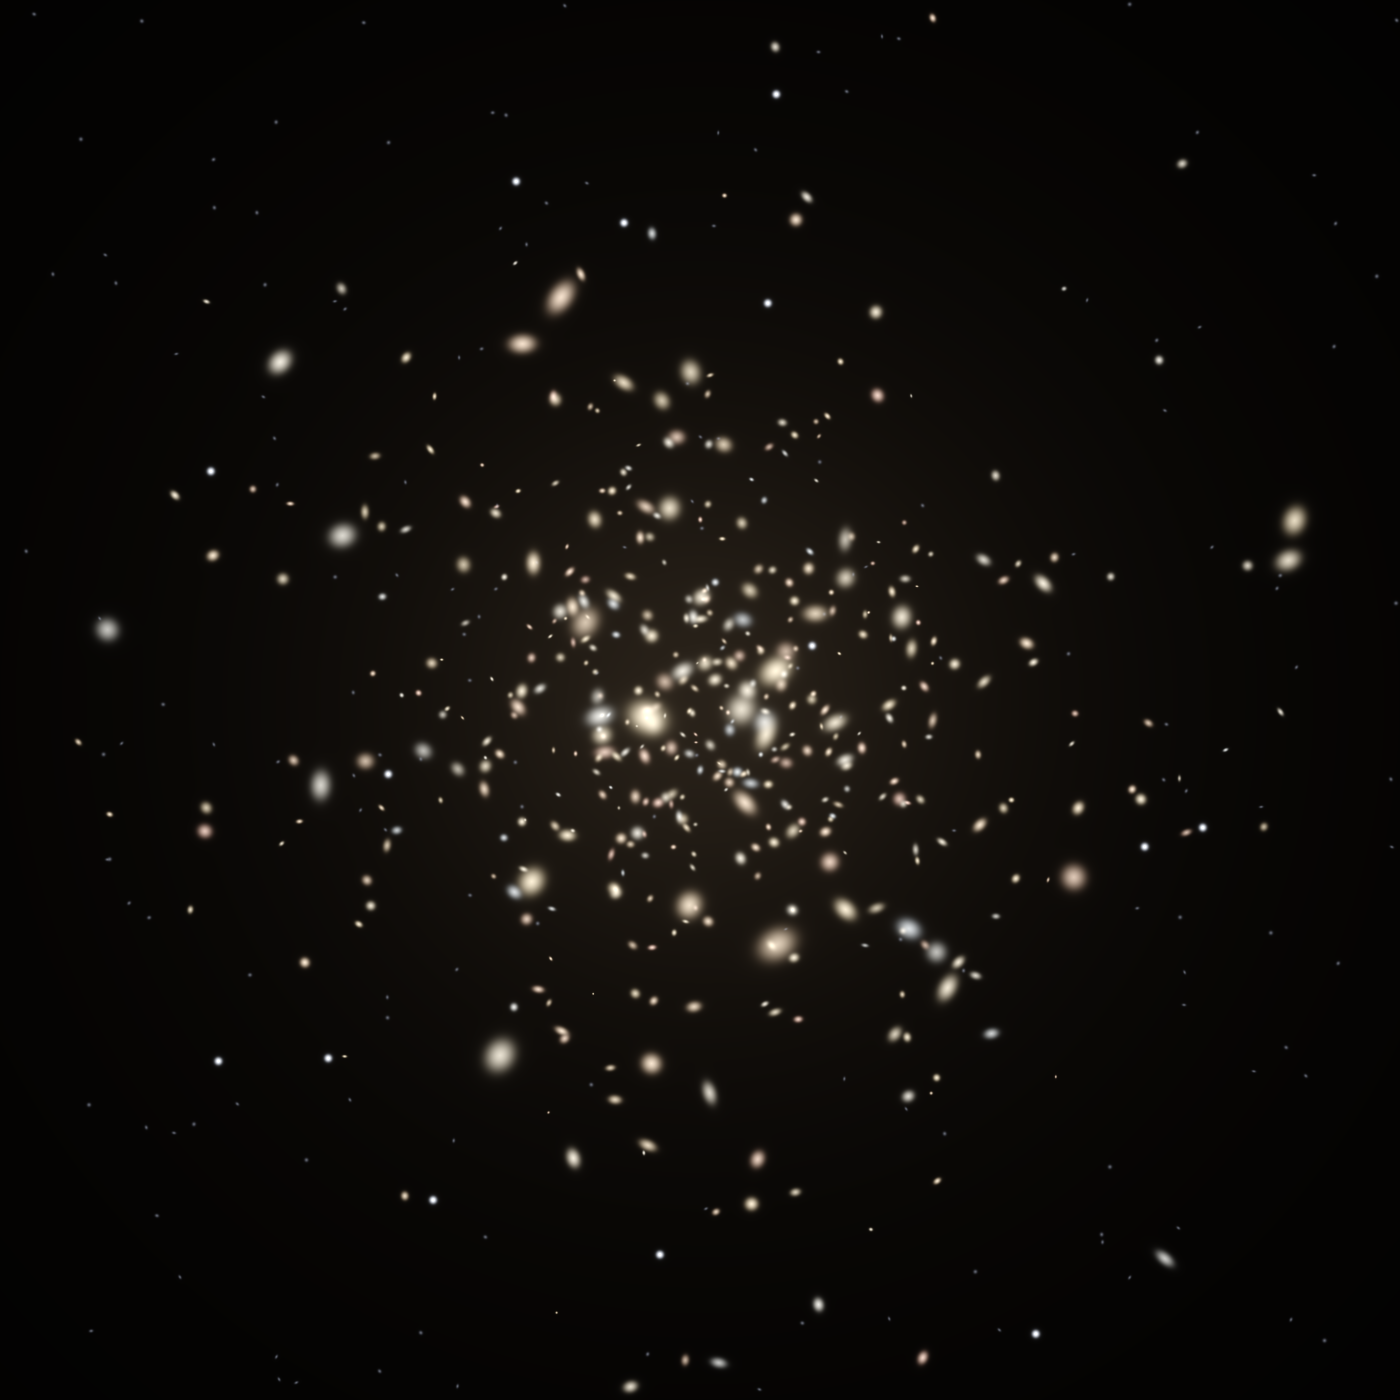
\includegraphics[width=6.0cm]{figs/cumulo.png}};
  \draw[cian!80,line width=0.5pt,dash pattern=on 2pt off 2pt] (0,0) circle (1.75);
  \draw[cian!80,line width=0.4pt,-{Stealth[length=3pt]}] (0,0) -- (-45:1.75);
  \node[cian,font=\small,anchor=north west,inner sep=2pt,fill=fondo,fill opacity=0.75,text opacity=1] at (-45:1.75) {$R$};
  \draw[texto!50,line width=0.4pt] (-3.0,-3.0) rectangle (3.0,3.0);
  \node[etiq,anchor=south] (ta) at (0,3.15) {(a) Cúmulo de galaxias};
  \node[peq,anchor=north,inner sep=3pt,align=center] at (0,-3.0)
    {tono: velocidad en la línea de visión};
\end{tikzpicture}\hspace{6mm}%
\begin{tikzpicture}[baseline=(tb.base)]
\begin{axis}[oscuro,width=7.4cm,height=7.0cm,
  xmin=0,xmax=30,ymin=0,ymax=240,
  xlabel={$r$ (kpc)},ylabel={$v$ (km/s)},
  legend pos=south east,legend cell align=left]
  \addplot[cian,line width=1.1pt,domain=0.3:30,samples=200]
    {sqrt(290526*(1-(1+x/3)*exp(-x/3))/x + 175^2*(1-5/x*rad(atan(x/5))))};
  \addlegendentry{total (con halo)}
  \addplot[ambar,dashed,line width=0.9pt,domain=0.3:30,samples=200]
    {sqrt(290526*(1-(1+x/3)*exp(-x/3))/x)};
  \addlegendentry{sólo masa visible}
  \addplot[only marks,mark=*,mark size=1.3pt,texto,error bars/.cd,y dir=both,y explicit,
    error bar style={texto!60,line width=0.4pt}]
    table[x=r,y=v,y error=e]{datos/rotacion.dat};
  \addlegendentry{observado}
\end{axis}
\node[etiq,anchor=south] (tb) at (2.55,5.95) {(b) Curva de rotación};
\end{tikzpicture}
\caption{(a) Representación esquemática de un cúmulo como Coma: el teorema del
virial, con la dispersión de velocidades (tono azulado o rojizo según el
corrimiento Doppler) y el radio $R$, da su masa total. (b) Curva de rotación de
una galaxia espiral (modelo ilustrativo): la masa visible predice una caída
kepleriana (ámbar), pero la velocidad observada se mantiene plana, lo que exige
un halo de materia oscura.}
\label{fig:materia-oscura}
\end{figure}
% ---------------------------------------------------------------------
